\section{Results, convergence monitoring, and model checking}


\subsection{Estimated bias toward the majority party}
\label{results}

\begin{figure}
\centering
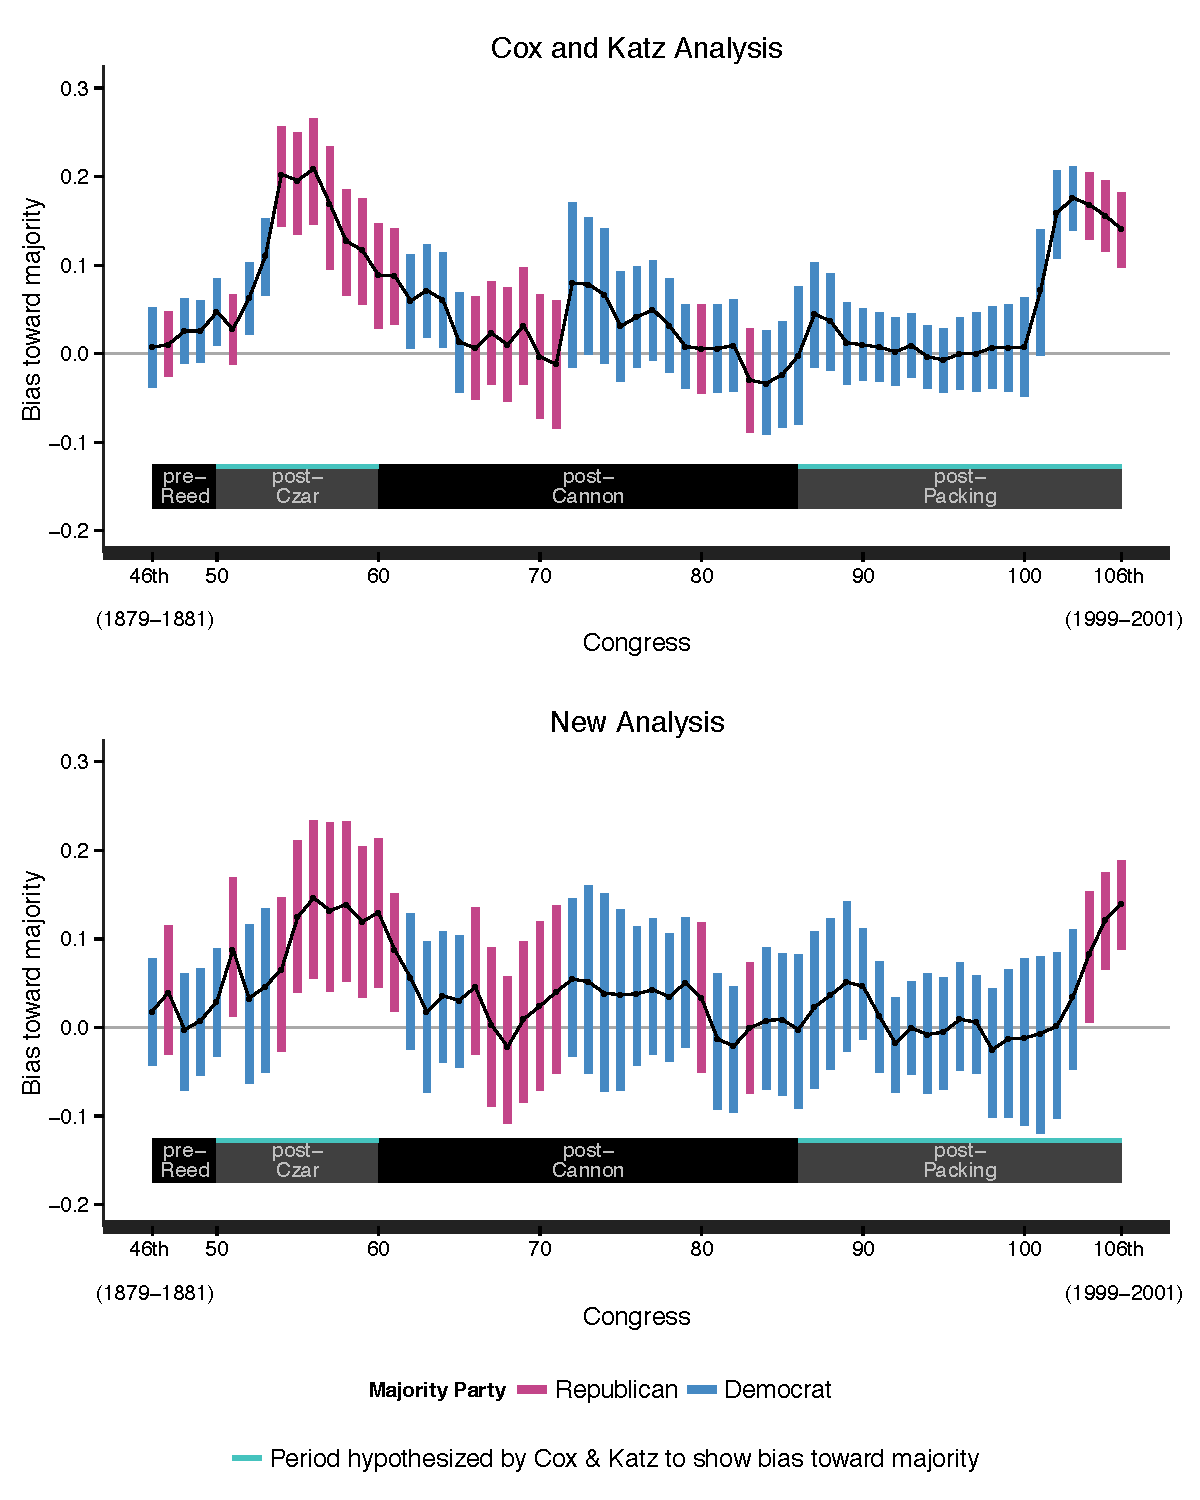
\includegraphics[scale=0.75]{sections/figs/ck_replication}
\caption{Estimated bias by Congress in Cox and Katz's analysis (top) and reanalysis (bottom). Vertical bars represent 95\%  intervals, with the black line connecting medians.}
\label{fig:ck_bias}
\end{figure}

Figure~\ref{fig:ck_bias} (p.~\pageref{fig:ck_bias}) shows the estimates of bias towards the majority party over time from Cox and Katz's analysis and the reanalysis conducted here. Immediately noticeable is the fact that the new estimates have greater uncertainties, which is to be expected due to the potential for Cox and Katz's method to produce overly precise estimates  (see section \ref{subsection_methods}). The new results do provide some support for the hypothesis of bias during the post-czar and post-packing periods, however the evidence is much weaker than that found by Cox and Katz. 

As discussed in \ref{subsection_methods}, Cox and Katz's analysis reuses the data for each Congress multiple times, but in the model for each Congress $t$ possibly relevant data from time periods outside its group of (up to) seven is excluded. The hierarchical Bayesian model, on the other hand, estimates a more believable trend in bias over time. This can be seen clearly by comparing the curves in Figure~\ref{fig:ck_bias}. The smoothing prior shrinks each individual estimate slightly towards its neighbors -- the amount of smoothing is related to the hierarchical variance hyperparameter -- which helps avoid the overfitting the data, while still allowing for substantial movement between Congresses if strongly supported by the data.  

\subsection{Convergence monitoring}
\label{subsection_convergence}

When making inferences using posterior simulations generated by an MCMC algorithm it is essential to check for evidence of convergence to the target distribution. Although this process is not an exact science, there is no shortage of literature on the topic of monitoring convergence for MCMC and other iterative simulation algorithms. The various convergence diagnostics used below are introduced informally. Formal definitions, computational details, and recommended best practices can be found in \citeA{gelman_handbook_2011}, \citeA{gelman_bayesian_2013}, and \citeA{stan_development_team_stan_2015}.

Eight randomly initialized chains of 500 iterations (after discarding 1000 warmup draws) were simulated.\footnote{Newcomers to HMC, NUTS, and Stan are often surprised by how few iterations are typically required, as it is not uncommon for Gibbs (and poorly tuned M-H) samplers to require hundreds of thousands of iterations to converge. Simpler models fit in Stan often require only hundreds of iterations, including warmup.} The distributions of three diagnostics calculated from the posterior sample are shown in Figure~\ref{fig:ck_diagnostics}. 

\begin{figure}[h]
\centering
	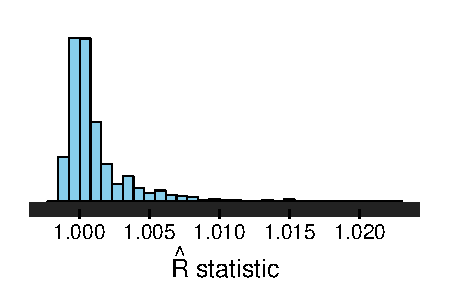
\includegraphics[scale=0.7]{sections/figs/rhat}
	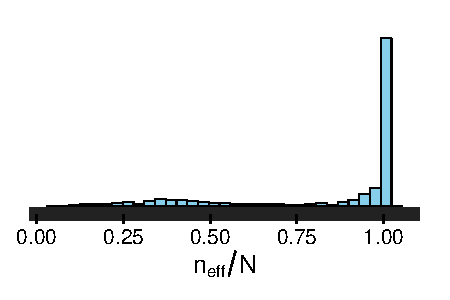
\includegraphics[scale=0.7]{sections/figs/neff}
	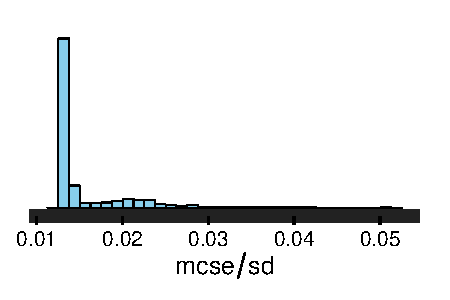
\includegraphics[scale=0.7]{sections/figs/mcse}
\caption{Distributions of diagnostics computed from the MCMC draws. From left to right: \newline ({\bf a}) Potential scale reduction factor $\hat{R}$ \newline ({\bf b}) Ratio of effective sample size to total sample size ($n_{\it eff}/N$) \newline ({\bf c}) Ratio of Monte Carlo error to posterior standard deviation ($mcse/sd$)}
\label{fig:ck_diagnostics}
\end{figure}

Figure~{\ref{fig:ck_diagnostics}a} shows the distribution of the estimates of the potential scale reduction statistic $\hat{R}$  \shortcite{gelman_rhat_1992}. The $\hat{R}$ statistic is a comparison of the variance of the simulations within individual chains to that of the simulations when chains are pooled. Here, the distribution of $\hat{R}$ shows that for all parameters the value is approximately one, indicating that little would be gained by running longer chains \shortcite{gelman_handbook_2011}. 

Figure~{\ref{fig:ck_diagnostics}b} shows the distribution of the ratio of effective sample size to the number of iterations ($n_{\it eff}/N$). Roughly speaking, $n_{\it eff}$ is an estimate of the number of {\it independent} draws from the posterior distribution that would have the same expected variance as the $N$ {\it dependent} draws actually obtained from the Markov chains. In this case $n_{\it eff}/N$ for all parameters is high and for most parameters the ratio is close to the ideal value of one, a reflection of Stan's efficiency. 


Figure~{\ref{fig:ck_diagnostics}c} shows the distribution of the ratio of Monte Carlo error to the estimated standard deviation ($mcse/sd$). Monte Carlo error is a measure of imprecision due to approximating the posterior distribution by the MCMC simulations. As the number of iterations increases $mcse$ goes to zero and the standard deviation of the draws converges to the posterior standard deviation. The distribution in Figure~\ref{fig:ck_diagnostics} shows that for all parameters the relative error $mcse/sd$ is less than five percent, which, for the inferential goals of this analysis is negligible. For instance, Figure~\ref{fig:ck_example_posterior} shows the estimated posterior density for the parameter corresponding to bias towards the majority party in the 79th congress.\footnote{There is nothing special about the 79th congress for this purpose. A single congress was chosen at random to use as an example.} The posterior is approximately Gaussian, with mean and standard deviation estimates of roughly $0.054$ and $0.0368$, respectively. The estimated $mcse$ is $0.0007$, which is inconsequential when compared to the uncertainty about the parameter in the posterior distribution.   


\begin{figure}[h]
\centering
	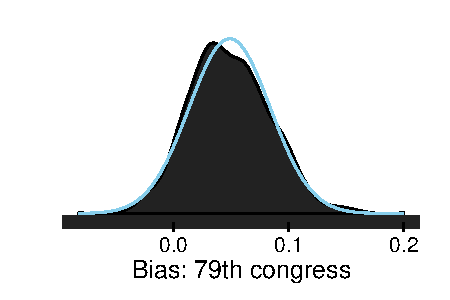
\includegraphics[scale=0.75]{sections/figs/example_posterior}
\caption{Posterior kernel density estimate for bias towards the majority party in the 79th congress. Normal density curve in blue.}
\label{fig:ck_example_posterior}
\end{figure}


%DEPENDENCE PLOT?
%
%
%\begin{figure}[h]
%\centering
%	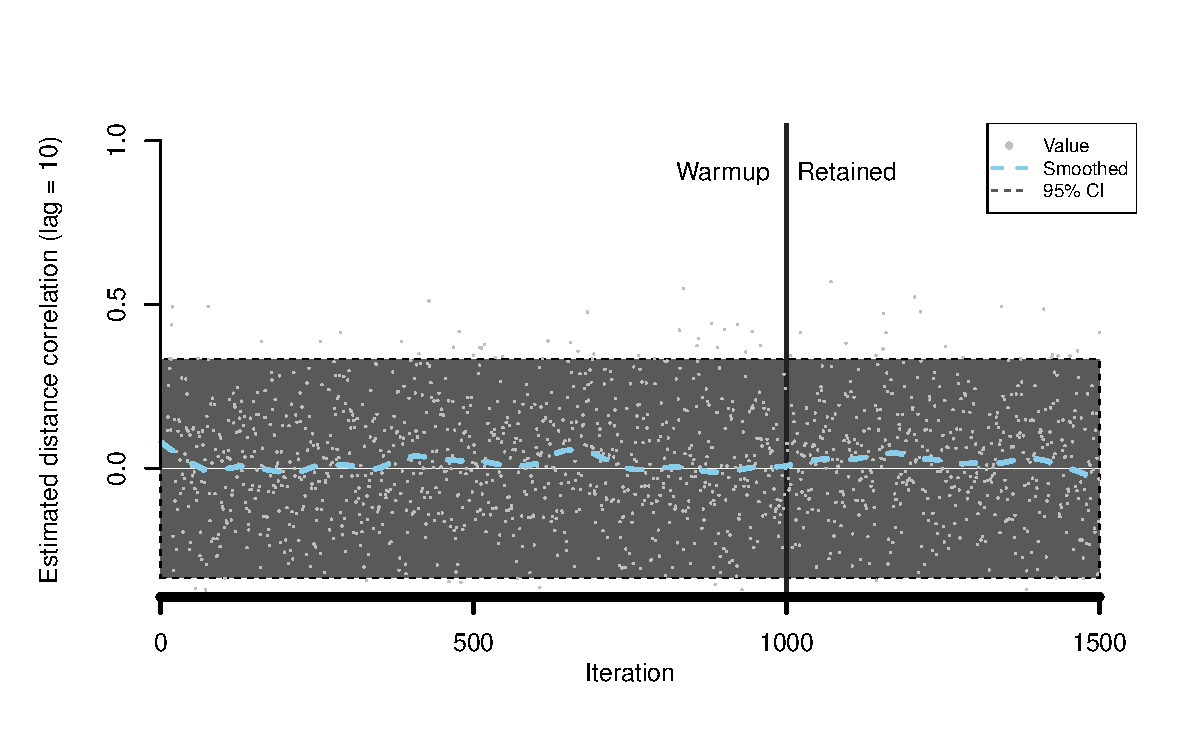
\includegraphics[scale=0.75]{sections/figs/ck_dependence}
%\caption{Estimated distance correlation among the eight chains. At a lag of 10 the draws are essentially independent. }
%\label{fig:ck_dependence}
%\end{figure}
%

In addition to the diagnostics discussed above, trace plots for all parameters were also examined as well as additional quantities specific to HMC and NUTS.\footnote{For example, checking that the tree depth used by NUTS is well below the user-specified maximum, ensuring that there are no post-warmup leapfrog iterations with diverging error, etc.}




\subsection{Graphical model checking}
\label{subsection_model_checking}

Graphical posterior predictive checking is a valuable tool for examining how well the proposed model fits the available data \shortcite{gelman_bayesian_2013}. The idea is simple: if the model is a good fit for the data then it should be possible simulate data from the model that resembles the data. Let $\Theta$ denote all parameters (including hyperparameters) in the hierarchical model, and $y$ denote the observed outcomes. Following the notation used by \citeA{gelman_bayesian_2013}, $y^{\it rep}$ will be used to denote a replication of $y$ from the model.\footnote{\citeA{gelman_bayesian_2013} distinguishes between $y^{rep}$ and $\tilde{y}$. The former makes use of the same explanatory variables/predictors $x$ used to estimate $\Theta$, while the latter refers predictions of future $y$ using potentially different variables $\tilde{x}$ (e.g. after collecting more data).}

For each draw of the parameters $\Theta$ from the posterior distribution $p(\Theta | y)$ an entire set of data $y^{\it rep} $ is simulated from the posterior predictive distribution

\begin{equation*}
 p(y^{\it rep} | y) = \int p(y^{\it rep} | \Theta) p(\Theta | y) d\Theta
\end{equation*}

\noindent which the likelihood for $y^{\it rep}$ averaging over the posterior distribution for $\Theta$. Thus, if we have $D$ draws of $\Theta$ from the posterior distribution and $y$ is an $N$-vector, then $D$ replicated data sets $y^{rep}$ will be simulated, each of which is also an $N$-vector.

The twelve histograms in Figure~\ref{fig:ck_pp_hists} (p. \pageref{fig:ck_pp_hists}) show the distribution of the observed data $y$ -- the number of roll-call votes won by the majority party -- alongside eleven replicated data sets $y^{\it rep}$ randomly selected from all of the posterior predictive replications. This is an informal comparison, but shows that indeed the observed data is plausible under the posterior predictive distribution implied by the model. It is an easy way of checking for inconsistencies due to poor model fit. Figure~\ref{fig:ck_pp_nWins_hists} (p. \pageref{fig:ck_pp_nWins_hists}) is similar to Figure~\ref{fig:ck_pp_hists} but shows the distribution of $y^{\it rep}$ by Congress. We can see that the observed data is consistent with the posterior predictive distribution. Finally, Figure~\ref{fig:ck_pp_test_statistics} (p. \pageref{fig:ck_pp_test_statistics}) shows the distributions of the mean and standard deviation over all replications, which nicely fit the observed values of these statistics in the data. 

% Should probably do pp checks after aggregating over the sub periods for each congress.  

\begin{figure}[h]
\centering
	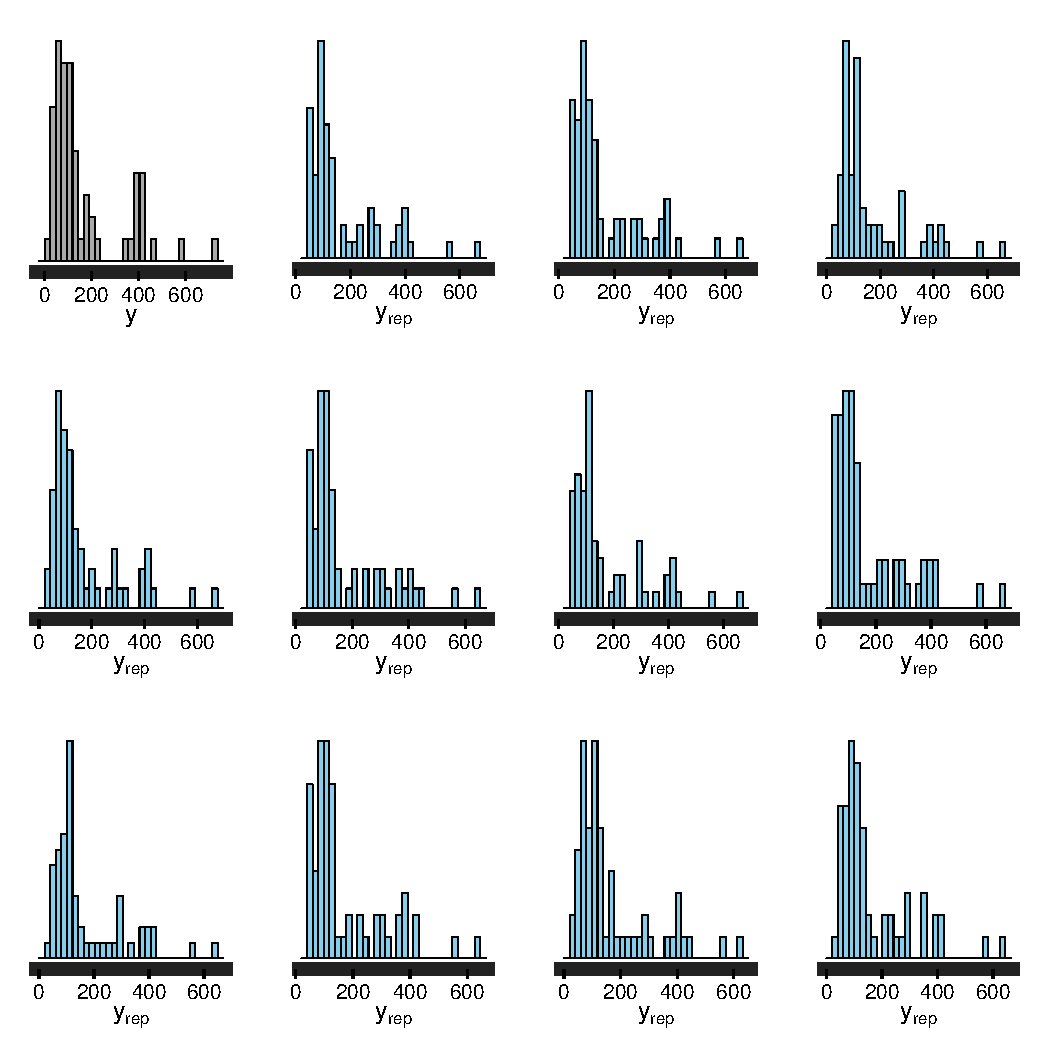
\includegraphics[scale=0.6]{sections/figs/ck_pp_y_vs_yrep_hists}
\caption{Replications from posterior predictive distribution vs. observed data}
\label{fig:ck_pp_hists}
\end{figure}

\begin{figure}[h]
\centering
	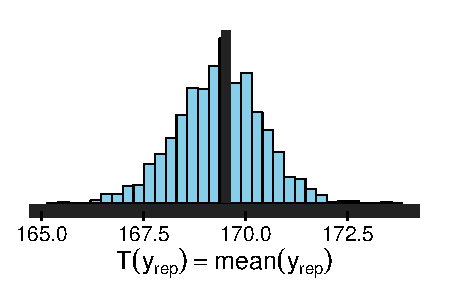
\includegraphics[scale=0.75]{sections/figs/test_stats_mean}
	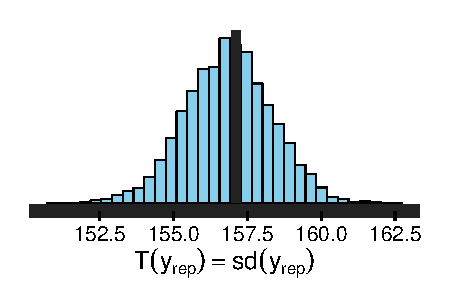
\includegraphics[scale=0.75]{sections/figs/test_stats_sd}
\caption{Distributions of test statistics $T(y_{rep})$. The vertical bar is the observed value $T(y)$.}
\label{fig:ck_pp_test_statistics}
\end{figure}

\begin{figure}
\centering
	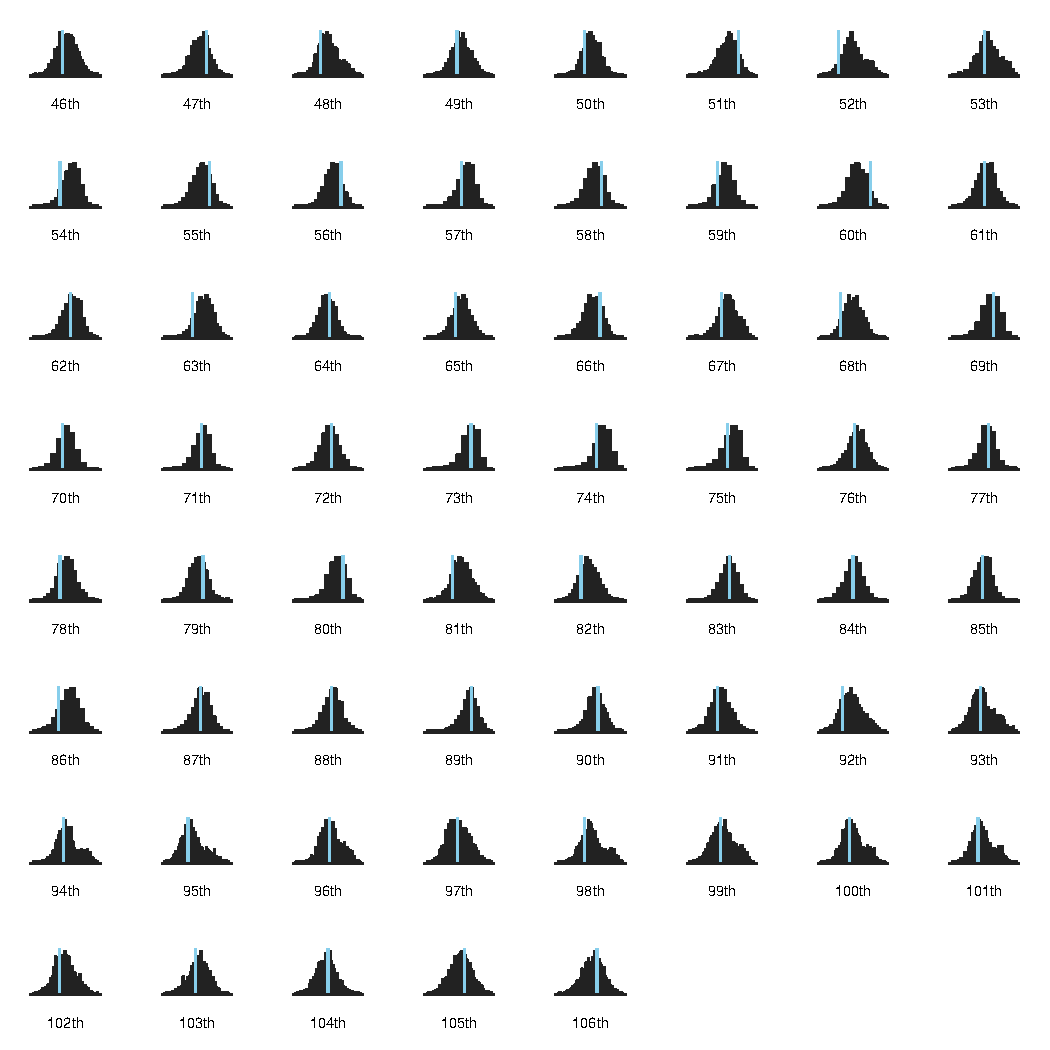
\includegraphics[scale=0.8]{sections/figs/ck_pp_nWins_hists}
\caption{Distributions of $y^{\it rep}$ by Congress. Vertical lines show observed values from the data.}
\label{fig:ck_pp_nWins_hists}
\end{figure}
